\documentclass[11pt]{article}
\usepackage[margin=1in]{geometry}
\usepackage{amsmath}
\usepackage{amssymb}
\usepackage{bm}
\usepackage{booktabs}
\usepackage{tikz}
\usepackage{xcolor}
\usepackage[colorlinks=true,linkcolor=blue,citecolor=blue]{hyperref}

\newcommand{\code}[1]{\texttt{\small #1}}
\newcommand{\file}[1]{\texttt{\footnotesize #1}}

\title{Bloch folding, supercells, and what \code{p2s\_map} actually does}
\author{Notes for the ACEWorkflow phonon pipeline}
\date{30 July 2026}

\begin{document}
\maketitle

\begin{abstract}
\noindent
Two different operations both get called ``folding'' in phonon calculations, and
conflating them is the usual source of confusion. This note separates them: the
\emph{Bloch transform}, which turns an infinite real-space problem into a small
$\bm q$-dependent eigenproblem, and \emph{zone folding}, which is what happens to
the band structure when you enlarge the unit cell. It then explains where
\code{p2s\_map}/\code{s2p\_map} enter (they are index bookkeeping for the first),
where the finite supercell introduces an approximation, and why only $16$ of the
$145$ band-path $\bm q$-points in this study are exactly represented.
\end{abstract}

%======================================================================
\section{The harmonic crystal and the Bloch transform}

Expand the total energy to second order in atomic displacements $\bm u$. Label a
primitive cell by its lattice vector $\bm R$, an atom within that cell by $i$,
and a Cartesian direction by $\alpha$:
%
\begin{equation}
E = E_0 + \frac12 \sum_{\bm R\bm R'}\sum_{ij}\sum_{\alpha\beta}
    u_{i\alpha}(\bm R)\,
    \Phi_{i\alpha,j\beta}(\bm R,\bm R')\,
    u_{j\beta}(\bm R'),
\label{eq:harmonic}
\end{equation}
%
with force constants $\Phi_{i\alpha,j\beta} = \partial^2 E/\partial u_{i\alpha}\partial u_{j\beta}$.
The equations of motion are
%
\begin{equation}
m_i\,\ddot u_{i\alpha}(\bm R)
  = -\sum_{\bm R' j\beta} \Phi_{i\alpha,j\beta}(\bm R,\bm R')\, u_{j\beta}(\bm R').
\label{eq:eom}
\end{equation}
%
This is an infinite system of coupled ordinary differential equations --- one per
atom per direction, over an unbounded crystal.

\paragraph{The fact that rescues it.} The crystal is invariant under lattice
translations, so $\Phi$ cannot depend on \emph{where} the pair sits, only on the
separation between the cells:
%
\begin{equation}
\Phi_{i\alpha,j\beta}(\bm R,\bm R') = \Phi_{i\alpha,j\beta}(\bm R' - \bm R).
\label{eq:translation}
\end{equation}
%
Equation~\eqref{eq:eom} is then a \emph{convolution} on the lattice, and
convolutions diagonalise under Fourier transform. Substituting the plane-wave
ansatz
%
\begin{equation}
u_{j\beta}(\bm R,t)
  = \frac{1}{\sqrt{m_j}}\, e_{j\beta}(\bm q)\, e^{i(\bm q\cdot\bm R - \omega t)}
\label{eq:ansatz}
\end{equation}
%
makes every explicit $\bm R$ cancel, leaving a finite eigenproblem at each
$\bm q$ separately:
%
\begin{align}
\omega^2(\bm q)\, e_{i\alpha}(\bm q)
  &= \sum_{j\beta} D_{i\alpha,j\beta}(\bm q)\, e_{j\beta}(\bm q),
\label{eq:eigen}\\[2pt]
D_{i\alpha,j\beta}(\bm q)
  &= \frac{1}{\sqrt{m_i m_j}}\sum_{\bm R}
     \Phi_{i\alpha,j\beta}(\bm R)\, e^{i\bm q\cdot\bm R}.
\label{eq:dynmat}
\end{align}
%
\textbf{The lattice sum in Eq.~\eqref{eq:dynmat} is the folding.} An infinite
problem has collapsed to a $3N_p \times 3N_p$ Hermitian matrix at each $\bm q$,
where $N_p$ is the number of atoms in the \emph{primitive} cell. For FCC
aluminium $N_p = 1$, so $\bm D(\bm q)$ is $3\times3$ and there are exactly three
branches at every $\bm q$: two transverse acoustic and one longitudinal.

In the code this is \file{src/Phonons/phonon\_bands.jl:121--154}. The lattice
vector $\bm R$ is built at line~130, the phase $e^{i\bm q\cdot\bm R}$ at
lines~139--140, and the mass normalisation $1/\sqrt{m_im_j}$ at line~145.

%======================================================================
\section{Why it is called ``folding''}

The wavevector $\bm q$ is not unique. A reciprocal lattice vector $\bm G$ is
defined by $e^{i\bm G\cdot\bm R} = 1$ for every lattice vector $\bm R$, so
%
\begin{equation}
e^{i(\bm q + \bm G)\cdot\bm R} = e^{i\bm q\cdot\bm R}
\qquad\Longrightarrow\qquad
\bm D(\bm q + \bm G) = \bm D(\bm q).
\label{eq:periodicity}
\end{equation}
%
Adding $\bm G$ produces a physically \emph{identical} displacement pattern. So
$\bm q$ is meaningful only modulo $\bm G$, and every wavevector outside the first
Brillouin zone \emph{folds back} into it. Physically: there is no phonon with a
wavelength shorter than the interatomic spacing. Attempting to specify one merely
re-describes a longer-wavelength mode, because the atoms only sample the wave at
discrete points.

\paragraph{What $\bm q$ means.} A wavevector is a \emph{phase relationship
between neighbouring cells}, nothing more. At $\bm q = \bm 0$ ($\Gamma$) every
cell moves identically, in lockstep. At a zone boundary, adjacent cells move
exactly out of phase. In between, there is a progressive phase shift --- a
travelling wave of wavelength $2\pi/|\bm q|$.

%======================================================================
\section{Zone folding: what happens when you enlarge the cell}

Now take a supercell of $N_{\mathrm{cell}}^3$ primitive cells instead of the
primitive cell itself. Its real-space lattice is coarser by $N_{\mathrm{cell}}$
in each direction, so its \emph{reciprocal} lattice is \emph{denser} by the same
factor and its Brillouin zone is smaller in volume by $N_{\mathrm{cell}}^3$.

Wavevectors that were ordinary interior points of the primitive zone are now
reciprocal lattice vectors \emph{of the supercell}, so by
Eq.~\eqref{eq:periodicity} they fold onto $\Gamma$. The three primitive branches,
sampled at the $N_{\mathrm{cell}}^3$ commensurate wavevectors, reappear as
$3N_{\mathrm{cell}}^3$ branches crammed into the smaller zone
(Fig.~\ref{fig:folding}).

\begin{figure}[h]
\centering
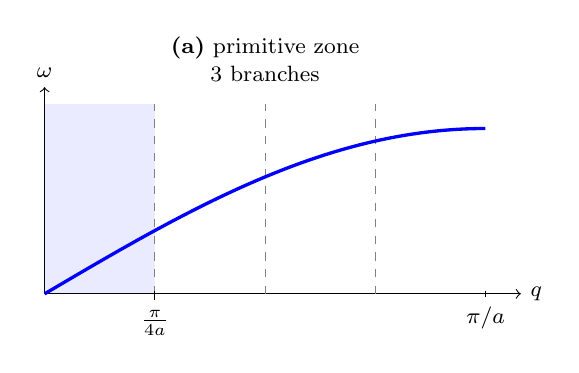
\begin{tikzpicture}[xscale=5.6, yscale=2.1]
  % --- Panel A: extended zone -------------------------------------------
  \fill[blue!8] (0,0) rectangle (0.25,1.15);
  \draw[->] (0,0) -- (1.08,0) node[right] {\footnotesize $q$};
  \draw[->] (0,0) -- (0,1.25) node[above] {\footnotesize $\omega$};
  \foreach \x in {0.25,0.5,0.75}
    \draw[gray,dashed] (\x,0) -- (\x,1.15);
  \draw[very thick,blue,domain=0:1,samples=80,smooth]
       plot (\x,{sin(90*\x)});
  \draw (1,0.02) -- (1,-0.02) node[below] {\footnotesize $\pi/a$};
  \draw (0.25,0.02) -- (0.25,-0.04) node[below] {\footnotesize $\tfrac{\pi}{4a}$};
  \node[align=center] at (0.5,1.42) {\footnotesize\textbf{(a)} primitive zone\\[-2pt]
        \footnotesize 3 branches};
\end{tikzpicture}
\hspace{0.6cm}
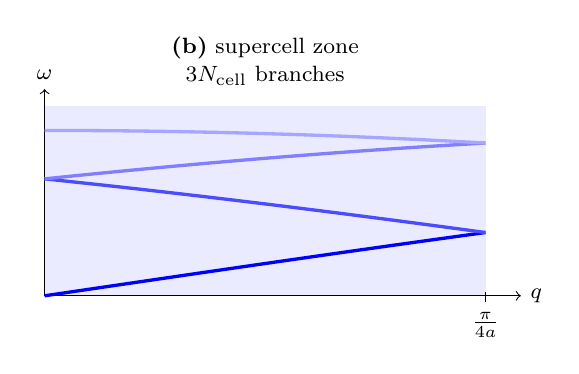
\begin{tikzpicture}[xscale=22.4, yscale=2.1]
  % --- Panel B: reduced (supercell) zone --------------------------------
  \fill[blue!8] (0,0) rectangle (0.25,1.15);
  \draw[->] (0,0) -- (0.27,0) node[right] {\footnotesize $q$};
  \draw[->] (0,0) -- (0,1.25) node[above] {\footnotesize $\omega$};
  \draw[very thick,blue,domain=0:0.25,samples=40,smooth]
       plot (\x,{sin(90*\x)});
  \draw[very thick,blue!70,domain=0:0.25,samples=40,smooth]
       plot (\x,{sin(90*(0.5-\x))});
  \draw[very thick,blue!50,domain=0:0.25,samples=40,smooth]
       plot (\x,{sin(90*(0.5+\x))});
  \draw[very thick,blue!35,domain=0:0.25,samples=40,smooth]
       plot (\x,{sin(90*(1-\x))});
  \draw (0.25,0.02) -- (0.25,-0.04) node[below] {\footnotesize $\tfrac{\pi}{4a}$};
  \node[align=center] at (0.125,1.42) {\footnotesize\textbf{(b)} supercell zone\\[-2pt]
        \footnotesize $3N_{\mathrm{cell}}$ branches};
\end{tikzpicture}
\caption{Zone folding in one dimension for $N_{\mathrm{cell}}=4$. (a) The
acoustic branch across the primitive Brillouin zone; dashed lines mark the
supercell zone boundaries. (b) The same physical content re-expressed in the
$4\times$ smaller supercell zone: each segment of (a) folds back into the shaded
region, producing four branches where there was one. No physics changes --- only
the labelling.}
\label{fig:folding}
\end{figure}

For the cells used in this study: the conventional cubic FCC cell holds 4 atoms,
so a $4\times4\times4$ conventional supercell holds $4\times4^3 = 256$ atoms,
i.e.\ 256 primitive cells. Its $\Gamma$ point therefore contains, superimposed,
the primitive modes at all 256 commensurate wavevectors:
%
\begin{equation}
3 \times 256 = 768 = 3N_{\mathrm{at}},
\end{equation}
%
which is exactly the dimension of the raw supercell Hessian.

\paragraph{The two operations are near-inverses.} Table~\ref{tab:two} states
them side by side. They carry the same physical content whenever $\bm q$ is
commensurate; they differ only in bookkeeping.

\begin{table}[h]
\centering
\caption{The two senses of ``folding'', and where each is implemented.}
\begin{tabular}{lll}
\toprule
 & Bloch transform & Zone folding \\
\midrule
direction      & real space $\to$ $\bm D(\bm q)$ & large BZ $\to$ small BZ \\
cell used      & true primitive cell             & supercell as its own cell \\
result (FCC Al, $4^3$) & 3 branches, $\bm q$ continuous & 768 branches at fixed $\bm q$ \\
implementation & \file{phonon\_bands.jl:121}     & \file{get\_hessian\_phonopy.jl:261} \\
\bottomrule
\end{tabular}
\label{tab:two}
\end{table}

%======================================================================
\section{What \code{p2s\_map} and \code{s2p\_map} are}

They are the index arithmetic that lets the lattice sum of
Eq.~\eqref{eq:dynmat} be run as a sum over \emph{supercell atoms}. Every
supercell atom is a lattice translate of exactly one primitive atom, which
partitions the $N_s$ supercell atoms into $N_p$ equivalence classes:
%
\begin{align}
\code{p2s\_map}[i] &: \text{primitive atom } i \;\longmapsto\;
  \text{index of its representative supercell atom},\\
\code{s2p\_map}[k] &: \text{supercell atom } k \;\longmapsto\;
  \text{index of \emph{that atom's} representative, also in supercell space.}
\end{align}
%
Note that \emph{both} take values in supercell index space. \code{s2p\_map} does
not return a number in $0,\dots,N_p-1$. That is precisely why the two can be
compared directly to select the images of a given primitive atom, as at
\file{phonon\_bands.jl:128}:
%
\begin{center}
\code{s2p\_map[k + 1] == j || continue}
\end{center}
%
which reads ``skip supercell atom $k$ unless it is a periodic image of primitive
atom $j$''. The sum that is actually evaluated is
%
\begin{equation}
D_{i\alpha,j\beta}(\bm q)
 = \frac{1}{\sqrt{m_im_j}}
   \sum_{k\,:\,\code{s2p}(k)=j}
   \bm H\big[\,3\,\code{p2s}(i)+\alpha,\; 3k+\beta\,\big]\;
   e^{i\bm q\cdot\bm R_k},
\qquad
\bm R_k = \bm r_k - \bm r_j .
\label{eq:implemented}
\end{equation}
%
The row index is pinned to a representative; the column sweeps over all images.
These maps are \emph{not} periodic boundary conditions --- they encode
translational symmetry, which an infinite crystal possesses regardless of any
boundary. In this repository they are constructed by explicit matching at
\file{phonon\_bands.jl:81--106}.

%======================================================================
\section{Where the finite supercell approximates}

Equation~\eqref{eq:dynmat} requires $\Phi(\bm R)$ for the infinite crystal, but a
supercell calculation with periodic boundaries returns the \emph{image sum}
%
\begin{equation}
\bm H[i,\,j+\bm R] \;=\; \sum_{\bm n} \Phi\big(\bm R + \bm n\cdot \bm L_{\mathrm{super}}\big),
\label{eq:imagesum}
\end{equation}
%
lumping together every periodic copy. The individual $\Phi(\bm R)$ is recovered
only if $\Phi$ has decayed to zero before the supercell boundary, so that exactly
one term in Eq.~\eqref{eq:imagesum} survives. This is the documented precondition
at \file{phonon\_bands.jl:52--54} and is the real constraint on
$N_{\mathrm{cell}}$.

\paragraph{How large is large enough.} For a site potential
$E = \sum_i \varepsilon_i$ with cutoff $r_c$, the Hessian has range $2r_c$, not
$r_c$: the cross term $\partial^2 E/\partial\bm r_a\partial\bm r_b$ is non-zero
whenever some site $i$ has \emph{both} $a$ and $b$ as neighbours. With
$r_c = 6$~\AA{} the force constants therefore extend to $\approx12$~\AA, while a
$4\times4\times4$ cell at $a = 4.045$~\AA{} has an edge of $16.2$~\AA{} and a
half-width of $8.1$~\AA. Strict image isolation would want an edge exceeding
$2\times 2r_c = 24$~\AA, i.e.\ $N_{\mathrm{cell}}\ge6$.

This gap is the standard situation in supercell phonon work and the residual
terms are far-tail and small, but it is an empirical question, not a provable
one. The check that settles it is convergence against a larger cell.

%======================================================================
\section{Consequence: interpolation and commensurability}
\label{sec:commensurate}

Because the force constants are known for a finite set of $\bm R$, evaluating
Eq.~\eqref{eq:dynmat} at an arbitrary $\bm q$ sums that finite set against an
arbitrary phase. This is \textbf{Fourier interpolation}: exact where $\bm q$ is
commensurate with the supercell, since there the finite $\bm R$-set is complete,
and interpolated everywhere else, with quality set by how fast $\Phi$ decays.

A finite box with periodic boundaries can only host waves that close on
themselves --- an integer number of wavelengths across the box:
%
\begin{equation}
\bm q\cdot\bm L_{\mathrm{super}} \in 2\pi\mathbb{Z}.
\label{eq:commensurate}
\end{equation}
%
Anything else would be discontinuous where the box wraps onto itself. Converting
a primitive-cell fractional wavevector $\bm f$ to conventional-cell fractional
coordinates,
%
\begin{equation}
\bm g = (-f_1+f_2+f_3,\;\; f_1-f_2+f_3,\;\; f_1+f_2-f_3),
\end{equation}
%
Eq.~\eqref{eq:commensurate} becomes the requirement that
$N_{\mathrm{cell}}\,\bm g \in \mathbb{Z}^3$.

Applying this to the band path $\Gamma\to X\to U\to L\to\Gamma\to K$ with
$[20,20,20,20,60]$ points per segment: of the 145 sampled wavevectors, only
\textbf{16 ($11.0\%$)} are commensurate with a $4\times4\times4$ cell. Per
segment the counts are $5/21$, $2/21$, $2/21$, $3/21$ and $4/61$. The remaining
129 are interpolated --- legitimate, and as good as the decay of $\Phi$, but not
independent data.

\paragraph{Why this matters for the constraint.} The same restriction applies to
any molecular-dynamics cell of the same size. A $4\times4\times4$ MD supercell
cannot host, and therefore cannot falsify, the $89\%$ of constrained modes that
are incommensurate with it. This is not a defect in the constraint: it means the
harmonic constraint acts on a finer $\bm q$-grid than the MD can resolve, so the
constraint is doing strictly more than the dynamics can check. A naive committee
member carrying imaginary modes at incommensurate $\bm q$ may nonetheless run as
a clean FCC crystal in that cell.

%======================================================================
\section*{Summary}

\begin{enumerate}
  \item Translational symmetry, Eq.~\eqref{eq:translation}, makes the equations
        of motion a convolution; Fourier transforming it gives the dynamical
        matrix Eq.~\eqref{eq:dynmat}. That sum is the Bloch folding, and it
        reduces an infinite problem to $3N_p\times3N_p$ at each $\bm q$.
  \item $\bm q$ is defined only modulo a reciprocal lattice vector, so
        wavevectors fold into the first Brillouin zone. Enlarging the cell
        shrinks that zone and folds the branches onto each other --- the same
        physics, more branches.
  \item \code{p2s\_map}/\code{s2p\_map} are the index bookkeeping for the sum in
        Eq.~\eqref{eq:implemented}. They encode translational symmetry, not
        periodic boundary conditions.
  \item The finite supercell enters through Eq.~\eqref{eq:imagesum}: individual
        force constants are recovered only once $\Phi$ has decayed within the
        box, which needs verifying against a larger cell rather than assuming.
  \item Off the commensurate grid, $\bm D(\bm q)$ is an interpolation. Only
        $16/145$ band-path points are exact at $N_{\mathrm{cell}}=4$, which is
        also why MD in a cell that size cannot test most of the constraint.
\end{enumerate}

\end{document}
